\chapter{Physics Objects\label{ch:objects}}

After data is selected by the trigger, the offline analyses begin with particle identification.
There are no longer any timing limitations, so such identifications can make use of all the detector
information in the event. CMS uses the Particle Flow (PF) algorithm in most analyses, which is
described in Section~\ref{sec:PF}.
As this search centers around the identification of events with both $\Hgg$ and $\Hbb$ decays, the
identification and reconstruction of photons and jets are the first steps taken after the
trigger selects potentially-interesting events,
and this chapter discusses the treatments needed at this stage for both data and MC samples.
Recalling that the sensitivity in the separation between signal and background comes from the
excellend diphoton mass resolution, the identification of two high quality photons is the starting point
and discussed in Section~\ref{sec:photons}. The following step is the identification of two jets
coming from the hadronization of b-quarks and is discussed in Section~\ref{sec:jets}.


\section{Particle Flow\label{sec:PF}}

The PF algorithm recontructs all stable particles in an event from the digitized electronic signals
of all channels in all subsystems~\cite{PFPAS2009,CMS-PAS-PFT-10-001}. These particles include
electrons, photons, charged hadrons, neutron hadrons, and muons, as shown in Figure~\ref{fig:PF}.


\begin{figure}[ht]
 \begin{center}
    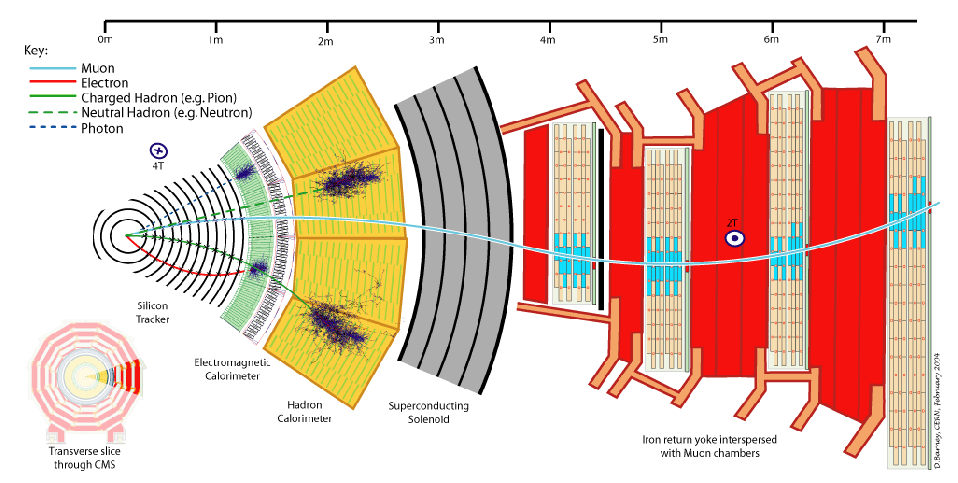
\includegraphics[width=0.95\textwidth]{figures/objects/pf.pdf}
      \end{center}
\caption{A schematic of a slice of the CMS detector in the plane transverse to the beam line.
The trajectories of an electron, photon, charged hadron, neutral hadron, and muon are superimposed
with the interactions that each of these particles would have with the various subsystems.}
\label{fig:PF}
\end{figure}


%Matching the muons to the tracks measured in the silicon tracker results in a transverse momentum
%resolution between 1 and 5\,\% for \pt values up to 1~TeV. The ECAL has an energy resolution better
%than 0.5\% for unconverted photons with transverse energies above 100~GeV.
%The HCAL, when combined with the ECAL, measures jets with a resolution
%$\Delta E/E \approx 100\,\% / \sqrt{E\,[\gev]} \oplus 5\,\%$.



\section{Photons\label{sec:photons}}
ref by this chapter

\section{Jets\label{sec:jets}}
reference by subsec:hcal
